\documentclass{article}


\PassOptionsToPackage{numbers, compress}{natbib}
\usepackage[preprint]{neurips_2020}
    
\usepackage[utf8]{inputenc} % allow utf-8 input
\usepackage[T1]{fontenc}    % use 8-bit T1 fonts
\usepackage{hyperref}	    % hyperlinks
\usepackage{url}	    % simple URL typesetting
\usepackage{booktabs}	    % professional-quality tables
\usepackage{amsfonts}	    % blackboard math symbols
\usepackage{nicefrac}	    % compact symbols for 1/2, etc.
\usepackage{microtype}	    % microtypography
\usepackage{xcolor}	    % text color
\usepackage{xspace}
\usepackage{amsmath}
\usepackage{amssymb}
\usepackage{graphicx}
\usepackage{caption}
\usepackage{subcaption}

% YZ: does this title work? feel free to change lol
\title{Collaborative Filtering for Music Recommendation}

% The \author macro works with any number of authors. There are two commands
% used to separate the names and addresses of multiple authors: \And and \AND.
%
% Using \And between authors leaves it to LaTeX to determine where to break the
% lines. Using \AND forces a line break at that point. So, if LaTeX puts 3 of 4
% authors names on the first line, and the last on the second line, try using
% \AND instead of \And before the third author name.

\author{
  Zander Meitus \qquad Yiming Zhang \\
  University of Chicago \\
  \texttt{\{zmeitus,yimingz0\}@uchicago.edu}
}

\newcommand{\aoty}{{\bf AOTY}\xspace}
\DeclareMathOperator{\X}{\mathit{X}}
\DeclareMathOperator{\U}{\mathcal{U}}
\DeclareMathOperator{\I}{\mathcal{I}}
\newcommand{\card}[1]{\ensuremath{\lvert {#1} \rvert}}
\newcommand{\easer}{$\text{EASE}^\text{R}$}
\newcommand{\userknn}{UserKNN\xspace}
\newcommand{\norm}[1]{\ensuremath{\lVert #1 \rVert}}
\newcommand{\transpose}[1]{{#1}^\mathsf{T}}
\newcommand{\yiming}[1]{\textcolor{violet}{[#1 ---\textsc{YZ}]}}
\newcommand{\zander}[1]{\textcolor{blue}{[#1 ---\textsc{ZM}]}}
\newcommand{\secref}[1]{\S\ref{#1}}

\begin{document}

\maketitle

\section{Introduction}

In this project, we study music recommendation using tools we learned in the
 class and Collaborative Filtering (CF) methods.
Collaborative Filtering performs matrix completion by leveraging user-level and
 album-level similarities: for a set of $n$ users and $p$ items, the user-item
 matrix $\X$ takes the form of $\X = \mathbb{R}^{n \times p}$, with potentially
 missing values when no rating is available.
Then, the recommendation problem boils down to identifying a set of ``good''
 items $\I_i$ for a user $i \in [n]$.

To study the problem of music recommendation, we create a new dataset (\aoty)
 as a testbed for music recommendation.
We chose two recommendation algorithms,
 \easer~\citep{steckEmbarrassinglyShallowAutoencoders2019} and
 \userknn~\citep{resnickGroupLensOpenArchitecture1994} to implement, for their
 state-of-the-art performance and computational tractability demonstrated by a
 recent survey~\citep{anelliTopNRecommendationAlgorithms2022}.
Then, we evalaute the recommendation performance of both algorithms on \aoty.
Both \easer and \userknn show strong recommendation performance on \aoty.
On a heldout test set, \easer achieves an F1@20 score of 27.0, an impressive
 score considering there are over 8k potential albums.
% Add a sentence for \userknn later.

\section{Method}
\zander{add lit review}
Collaborative Filtering, the technique of inferring the preferences of one user
 using known information about other users, is the dominant class of algorithm
 for recommendation systems.
In this project, we plan to implement, extend and evaluate two CF algorithms,
 \easer and \userknn, demonstrated as among the state-of-the-art in a
 comprehensive study by \citet{anelliTopNRecommendationAlgorithms2022}.

\paragraph*{\easer.}
\easer~\citep{steckEmbarrassinglyShallowAutoencoders2019}
is a linear model parameterized by a item-item matrix $B \in
	\mathbb{R}^{p \times p}$.
The weights $B$ are optimized with respect to the simple objective
 \begin{equation} \min_B \norm{\X - X B}_F^2 + \lambda \cdot \norm{B}_F^2
 \text{.
}
\end{equation}
Intuitively, \easer reconstructs user preferences using information about items
 exclusively.
In addition, \easer adds an matrix norm penalty, encouraging $B$ to be
 low-rank.

$B$ admits a degenerate solution $B = I$, under which the
recommendation system always recommends items that the user
already likes.
To avoid this solution, the author added an additional constraint that
 $\mathrm{diag}(B) = \mathbf{0}$.
Learning the weights of $B$ is a (constrained) convex optimization problem, and
 the optimal solution is given by  \begin{equation} \hat{B}_{i, j} =
	 \begin{cases} 0 & \text{if $i = j$} \\ -\frac{\hat{P}_{i, j}}{\hat{P}_{j, j}} &
               \text{otherwise,}     \\\end{cases} \end{equation} where $\hat{P} =
	 (\transpose{X} X + \lambda I)^{-1}$.

While the original work by \citet{steckEmbarrassinglyShallowAutoencoders2019}
 proposes a closed-form solution, computing this closed-form solution requires
 inverting an $p \times p$ matrix, taking $\mathcal{O}(p^3)$ time in a typical
 commercial implementation.
To save computational cost, we experiment with mini-batch stochastic gradient
 descent as an alternative technique for computing $B$.
To compute the loss $\min_B \norm{\X - X B}_F^2 + \lambda \cdot \norm{B}_F^2$,
 we need to multiply matrices $X$ and $B$.
Taking advantage of the sparsity of $X$, we can compute $X B$ in $\mathcal{O}(x
	 p)$ time, where $x$ is the number non-zero elements in $X$.
Then, this alternative training procedure takes $\mathcal{O}(kxp)$ time, where
 $k$ is the number of iterations until convergence.

\paragraph*{\userknn.}
\yiming{add some stuff here?}
Neighborhood-based recommendation methods essentially treat the preference of a
 user $u$ as a weighted sum of preferences of other users under some notion of
 similarity.
For a pair of users $u, v$,
 \userknn~\citep{resnickGroupLensOpenArchitecture1994} measures the similarity
 between users with the correlation coefficient $r_{uv}$ between items that $u$
 and $v$ both rated.
The predicted score for an item is the weighted sum of ratings of similar
 users, after adjusting for the ``baseline rating'' that the user gives to an
 average item.
 \begin{equation}
 P = \vec{\mu} + \frac{(A - \bar J)R}{M|R|}
 \end{equation}

$P$ is prediction matrix of $n$ albums and $p$ users. $\mu$ is the average rating
 of each reviewer. $A$ is the provided $nxp$ ratings matrix. $\bar J$ is an $n$ by $p$
 matrix where the $i,j$ entry is the average rating of the $j$th reviewer, exluding the $i$th
 rating. $R$ is the reviwer correlation matrix with diagonals set to 0. $M$ is a mask of
 $A$, where cells with ratings in $A$ are $1$ in M, and all other values of $M$ are 0. 
 The approach is heuristic in that there is no loss function to optimize or parameters
 to tune. The algorithm is simply run on the data to produce predictions.

\section{Experimental Setup}
\label{sec:setup}
\paragraph*{Data curation.}
For this project, we have created a dataset of album reviews, named \aoty, by
 scraping data from \url{https://www.albumoftheyear.org}.
On this website, users create profiles and rank albums from 0 to 100.
After filtering out albums with $<100$ total reviews and users with $<10$
 positive reviews, \aoty has a total of $8,855$ albums and $22,167$ users.
The average album in the dataset has $426.8$ reviews.
The user-album matrix is very sparse: for \aoty, the sparsity $s = 1.9 \times
	 10^{-2}$.
The {\em data sparsity} problem~\citep{suSurveyCollaborativeFiltering2009} in
 the user-item matrix is a major challenge in most real-world recommendation
 problems, and we believe this property makes \aoty a suitable testbed for
 studying recommendation.

\paragraph*{Evaluation settings and metrics.}
We consider two evaluation settings: {\em weak generalization}, where the
 recommendation algorithm is evaluated by a subset of all user-item
 interactions, and {\em strong generalization}, where the recommendation
 algorithm is evaluted on a heldout random subset of users. 
 \zander{also mention explicit vs. implicit?}

In weak generalization, a random subset of ratings are omitted from the user-rating
 matrix $X$ to create a user-rating matrix $X^{\prime}$. The algorithm is then run on 
 $X^{\prime}$ to generate predictions. The predictions for the omitted ratings are then 
 compared to the true ratings to evaluate performance.

  We evaluate \easer, both the original version and the gradient descent version
 in the strong generalizaton setting.
We report performance on a set of common retrieval metrics: Precision (P), Recall
 (R) and F1 @ $k$.
Precision @ $k$ measures the percentage of recommended items that user like in
 top-$k$ recommendations, and recall @ $k$ measures the the coverage of all
 items liked by a user in top-$k$ recommendations.
F1 @ $k$ is computed as the harmonic mean of precision and recall @ $k$.

Beyond these common retrieval metrics, we consider the following evaluation
 metrics following \citet{anelliTopNRecommendationAlgorithms2022}:
 \begin{itemize} \item {\em Item Coverage}: Item Coverage (IC) measures the
 percentage of distinct items that is recommended to at least one user.
\item {\em Gini}: Gini coefficient of the distribution of recommended items
measures the concentration of recommendation.

\end{itemize}

We evaluate \userknn in the weak generalization setting on the full user-rating matrix, 
omitting a random sample of 20\% of the ratings for a total of 736,944 test predictions.  
We also evaluate \userknn in the strong generalization setting. To apply strong 
generalization to \userknn, a new rating matrix needs to be generated for each test user that is $n$ by $v$, where $v$ is 
the number of valid ratings provided by the user. In each column, one of the valid values 
 is omitted so that the predicted value is not included in the correlation between
the test user and all training users. A correlation matrix $R_j$ for the $j$ test user
 then needs to be
calcualted between each column vector of the $j$th test user's matrix and the training matrix
$A$. Because this is computationally expensive to regenerate the correlation matrix, we 
 used only 10 random test users to
 evaluate \userknn in the strong generalization setting with a total of 1,121 predicted
 ratings.  

\userknn takes explicit feedback (ratings) as an input and generates explicit ratings as an output,
so we evaluate the model on mean absolute error (MAE) and root mean squared error (RMESE).
We also convert the true and predicted ratings to implicit feedback following the same
procedure as for \easer and evaluate on a set of common retrieval metrics: Precision (P), 
Recall (R) and F1 @ $k$. In the weak generalization test setting, test predictions are 
distributed across users randomly, so instead of evaluating @ top-$k$ for each user, we evaluate
the predictions as a whole. 



\section{Results}

\begin{figure*}[h]
	\centering
	\begin{subfigure}[b]{0.4\textwidth}
		\centering
		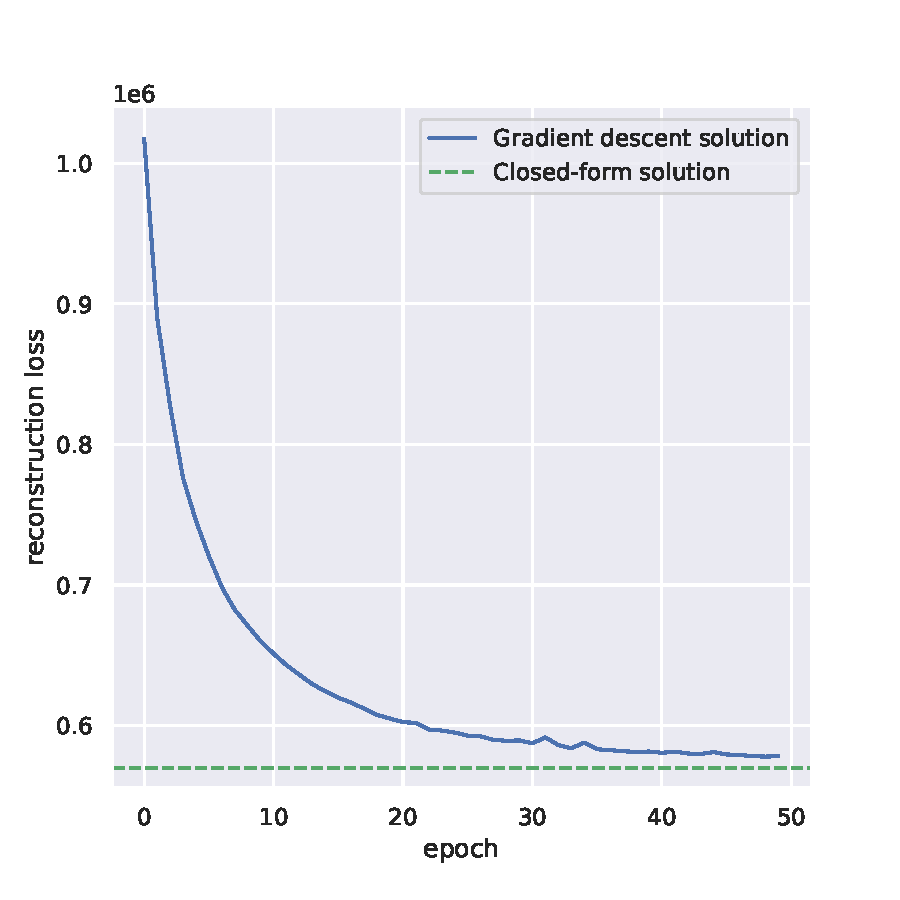
\includegraphics[width=\textwidth]{figures/recon-loss.pdf}
		\caption{Convergence of stochastic gradient descent to optimal
			solution in \easer.}
		\label{fig:convergence}
	\end{subfigure}
	% \hfill
	\begin{subfigure}[b]{0.4\textwidth}
		\centering
		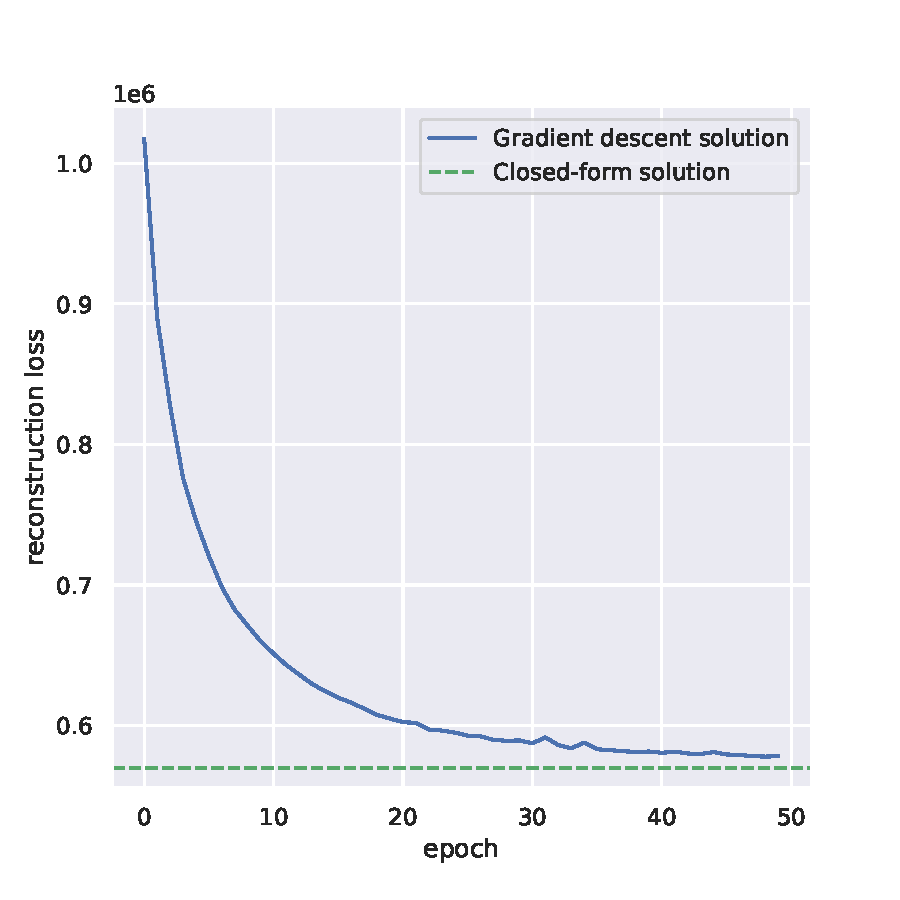
\includegraphics[width=\textwidth]{figures/recon-loss.pdf}
		\caption{\yiming{placeholder for new figures}.}
	\end{subfigure}
	\caption{}
	\label{fig:1}
\end{figure*}

\begin{table*}[h]
	\centering
	\begin{tabular}{@{}llll@{}}
		\toprule
		Evaluation metrics @ $20$     & \easer (closed-form) & \easer
		(SGD)
		\\ \midrule
		Precision $\uparrow$          & $69.2$               & $69.2$
		\\
		Recall	$\uparrow$              & $21.0$               &
		$21.0$
		\\
		F1	$\uparrow$                  & $27.0$               &
		$27.0$
		\\
		Item Coverage	$\uparrow$       & $34.7\%$             &
		$34.7\%$
		\\
		Gini	$\downarrow$              & $0.925$              &
		$0.925$
		\\
		Optimization time	$\downarrow$ & 5 seconds
		                              & 107 seconds
		\\ \bottomrule
	\end{tabular}
	\caption{Evaluation of top-20 recommendations of \easer on a heldout
		test set. $\uparrow$ means higher is better, and $\downarrow$
		means
		lower is better.}
	\label{tab:easer-results}

\end{table*}

\paragraph*{\easer.}
As discussed in \secref{sec:setup}, we evaluate the both the closed-form
 version of \easer and our proposed SGD approach on a heldout out test set of
 users.
We are interested in quantifying the recommendation quality of both algorithms,
 and also understanding whether our proposed approach produces a solution that
 converges to the closed-form solution.

One way to understand the convergence behavior of the algorithm is by measuring
 the reconstruction loss $\norm{X - X \hat{B}}_F^2$.
In Figure \ref{fig:1}\ref{sub@fig:convergence}, we plot the reconstruction loss
 corresponding to $\hat{B}^{(t)}$, the weights at epoch $t$, against the number
 of epochs $t$.
The green line corresponds to the reconstruction loss of the optimal
 closed-form solution.
We find that the reconstruction loss of stochastic gradient descent indeed
 converges to that of the closed-form solution.
This observation isn't surprising given that \easer has a convex objective, and
 gradient descent provably converges for convex objectives.
That said, SGD-based optimization takes 107 seconds in our experiment, 21x
 longer than that of computing the closed-form solution directly.
We suspect that although our proposed solution has smaller big-$\mathcal{O}$
 complexity on paper, it's not well-tuned compared  NumPy's matrix inversion
 algorithm.
In addition, multiplying with sparse matricies does not take advantage of cache
 locality, an important reason why accessing succesive locations in arrays are
 fast.

\easer shows strong recommendation performance when evaluated on unseen users
in training, highlighted by a Precision @ $20$ score of $69.2$, meaning users
provided
positive reviews for the majority of items we recommended.
While the Recall @ $20$ score is only $21.0$, the cutoff is smaller than the
 average number of reviews per user, making a perfect score unattainable.
Additionally, we argue that Precision is the more relevant metric in the
 recommendation problem, as we care mostly about recommending some, rather than
 all, items that a user will like.
We observe significant concentration in the recommendations of \easer, with
 roughly one-third of all albums recommended to at least one user.
The Gini score of $0.925$ highlights a strong inequality in the recommendation,
 with a small subset of albums being heavily favored over the rest.

\paragraph*{\userknn.} 
\yiming{todo}.

\section{Qualitative Analysis}

\newpage
\bibliography{ref,yiming}
\bibliographystyle{abbrvnat}
\end{document}